\documentclass{article}
\usepackage{tikz}
\usetikzlibrary{positioning}

\begin{document}

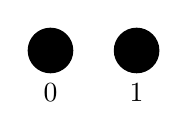
\begin{tikzpicture}[node distance=0.5cm]
    \node[circle,fill,inner sep=2pt,label=below:$0$] (v0) {$v_0$};
    \node[circle,fill,inner sep=2pt,right=of v0,label=below:$1$] (v1) {$v_1$};
\end{tikzpicture}

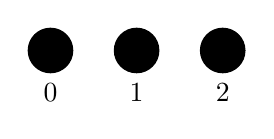
\begin{tikzpicture}[node distance=0.5cm]
    \node[circle,fill,inner sep=2pt,label=below:$0$] (v0) {$v_0$};
    \node[circle,fill,inner sep=2pt,right=of v0,label=below:$1$] (v1) {$v_1$};
    \node[circle,fill,inner sep=2pt,right=of v1,label=below:$2$] (v2) {$v_2$};
\end{tikzpicture}

\end{document}